\documentclass[11pt]{article}
\usepackage[a4paper,margin=2.5cm]{geometry}
\usepackage[T1]{fontenc}
\usepackage[utf8]{inputenc}
\usepackage{lmodern}
\usepackage{amsmath,amssymb}
\usepackage{booktabs}
\usepackage{tikz}
\usetikzlibrary{arrows.meta,positioning}
\usepackage[hidelinks]{hyperref}

\newcommand{\E}{\mathbb{E}}
\newcommand{\rn}{\operatorname{ranknorm}}
\newcommand{\med}{\operatorname{median}}
\newcommand{\code}[1]{\texttt{#1}}

\title{Domain-aware heterogeneous quantization\\and causal sub-network probes}
\author{\code{pretty\_duck}, branch \code{feature/domain-compression}}
\date{}

\begin{document}
\maketitle

\begin{abstract}
We describe a pipeline that (i) collects per-domain activation statistics of a language model,
(ii) plans a heterogeneous quantization of its linear layers under a byte budget, and
(iii) writes the plan as real packed weights with a measured manifest. On top of the
statistics we add causal probes (ablation and minimal-pair activation patching) that ask whether
channels selected by a domain contrast are \emph{used} by the model, rather than merely more
active on that domain. The results so far are mixed and are reported as measured. At block and
row-group granularity the domain signal is too weak to change an allocation. Per input channel
it is reproducible, but a mean-ablation effect that looks selective is fully explained by the
size of the perturbation. On Persona-style prompt pairs, however, a mean-difference channel
selector finds channels that are both sufficient and necessary for the prompt-induced margin
shift, beyond random and beyond a lexical control. Quantizing those channels at 3--4 bits does not
damage that behavior more than quantizing random channels of the same cost.
\end{abstract}

\section{Overview}

The pipeline has three stages (Figure~\ref{fig:pipeline}). This document covers the first two and
the converter's storage format; the final inference pipeline is out of scope. No gradients, auxiliary
networks or fine-tuning are used anywhere, and every probe is forward-only.

\begin{figure}[h]
\centering
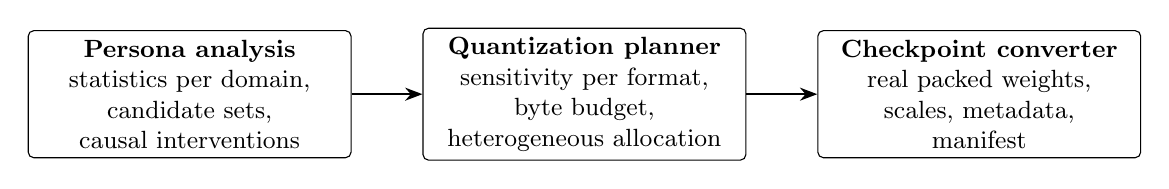
\begin{tikzpicture}[
  box/.style={draw, rounded corners=2pt, align=center, minimum width=4.1cm, minimum height=1.5cm, font=\small},
  arr/.style={-{Stealth[length=2.2mm]}, thick}]
  \node[box] (a) {\textbf{Persona analysis}\\statistics per domain,\\candidate sets,\\causal interventions};
  \node[box, right=0.9cm of a] (b) {\textbf{Quantization planner}\\sensitivity per format,\\byte budget,\\heterogeneous allocation};
  \node[box, right=0.9cm of b] (c) {\textbf{Checkpoint converter}\\real packed weights,\\scales, metadata,\\manifest};
  \draw[arr] (a) -- (b); \draw[arr] (b) -- (c);
\end{tikzpicture}
\caption{The three stages. The causal probes of Section~\ref{sec:probes} belong to the first stage;
only candidate sets that survive them would be passed to the planner.}
\label{fig:pipeline}
\end{figure}

\section{Statistics and local quantities}
\label{sec:stats}

Let $g$ index the \code{nn.Linear} layers of the text tower, $W_g\in\mathbb{R}^{o\times i}$ the weight
and $h_g(x)\in\mathbb{R}^{i}$ its input. For a domain $d$ with calibration set $C_d$ we accumulate, over
valid (non-padding) tokens and in double precision, three per-input-channel moments:
\begin{equation}
A_{g,d,j}=\E\,|h_{g,j}|,\qquad V_{g,d,j}=\E\,h_{g,j}^2,\qquad M_{g,d,j}=\E\,h_{g,j}.
\end{equation}
Hooks are removed on exit, also after an exception; tied heads and non-text towers are skipped.
The per-block importance and the diagonal quantization-error estimate are
\begin{align}
I_{g,d} &= \sum_{i,j} |W_{g,ij}|\,A_{g,d,j},\\
D_{g,d}(b) &= \sum_{i,j}\bigl(W_{g,ij}-Q_b(W_{g,ij})\bigr)^2\,V_{g,d,j}\;\approx\;\E_{x\sim C_d}\bigl\|x\,E_g^{(b)\top}\bigr\|_2^2 ,
\end{align}
where the last step assumes uncorrelated input channels. $D$ is a local prioritization signal, not a prediction of
the final loss: errors in different layers are not equally harmful, and the sum over layers is not the
loss increase.

\section{Quantization planner}
\label{sec:planner}

\paragraph{Formats and real bytes.}
Four portable formats are supported, all quantizing each output row independently:
\code{fp16}; \code{int8} and \code{int4} (symmetric, one fp16 scale per row); and \code{nf4}
(NF4 codebook, one fp16 absmax per 64-weight block of a row). The allocator uses exact payload formulas,
asserted against the packed tensors, never nominal bits per parameter: for a $(o,i)$ weight,
$B(\code{int8})=oi+2o$, $B(\code{int4})=\lceil oi/2\rceil+2o$ and $B(\code{nf4})=o\lceil i/64\rceil\,(32+2)$.

\paragraph{Greedy allocation.}
Every unit starts at \code{fp16}. A reduction $b\to b'$ of a unit $g$ that saves bytes has cost
\begin{equation}
\rho_{g,b\to b'}=\frac{D_{g,T}(b')-D_{g,T}(b)}{B_g(b)-B_g(b')},
\end{equation}
and the smallest $\rho$ is applied until a size budget is met, or until no reduction fits an error budget.
Steps that save no bytes or give a non-finite $\rho$ are skipped. The plan is a reproducible JSON file,
separate from its application to a model. Greedy selection is optimal only on the lower convex hull of each
block's (bytes, error) points, which is not guaranteed.

\paragraph{Row-group units.}
A unit is a whole layer or a group of consecutive output rows, named \code{layer@r0:r1}. Because each format
treats rows independently, a group quantized on its own is bit-identical to the same rows inside the full
matrix, and its bytes are exactly $B((r,i),b)$; this is checked by tests, including odd widths where int4 rows
share a byte. The converter regroups units into one file per layer and rejects groups that do not tile the layer.

\paragraph{Contrast signals.}
Two auxiliary signals can multiply $\rho$. The first uses $C_g=I_{g,T}-\lambda\,\overline{I_{g,S}}$, min--max
normalized over blocks. The second, \emph{target-anchored relative contrast} (TARC), ranks each domain across units,
$R_d(g)=\rn(I_d(g))\in[0,1]$ (average ranks for ties), and takes
\begin{equation}
S_T(g)=R_T(g)-\med_{d\neq T}R_d(g)\in[-1,1].
\end{equation}
Block size and layer type move every domain's rank the same way and cancel in the difference; the penalty is
$\rho\leftarrow\rho\,(1+\lambda\max(S_T,0))$, so $\lambda$ is only a strength. Both are hypotheses about
prioritization: the error term already contains the domain through $V_{g,T}$, and only evaluation can say whether
the contrast adds anything.

\section{Causal probes}
\label{sec:probes}

Statistics say a channel is more active on a domain; they do not say the model needs it. The probes intervene.

\subsection{Candidate channel sets}
For each layer a fraction $k$ of its $i$ input channels is selected by one of:
\begin{itemize}\setlength\itemsep{0pt}
\item \textbf{tarc}: top channels by $S_T$ computed from the per-channel $A_{d,j}$ ranks within the layer;
\item \textbf{zdiff}: top channels by $|M_{T,j}-\overline{M}_{o,j}|\big/\sqrt{\mathrm{var}_{T,j}+\overline{\mathrm{var}}_{o,j}}$,
 with $\mathrm{var}=V-M^2$ and bars denoting the mean over the other domains (the standardized mean difference);
\item \textbf{importance}: top channels by $A_{T,j}$ alone; \textbf{anti}: bottom channels by $S_T$;
\item \textbf{random}: same size, disjoint from a reference set, matched channel by channel on the $V$-rank;
\item \textbf{energy-random}: same size, disjoint, matched on the pair $(\log e^T_j,\log e^o_j)$ defined next.
\end{itemize}

\subsection{Mean ablation and the dose confound}
Replacing channel $j$ by a value $m_j$ (the mean of the other domains' $M$) perturbs the input by an expected squared amount
$e_j=\E(h_j-m_j)^2=V_j-2m_jM_j+m_j^2$ on each domain. A set chosen because the target differs from the others
perturbs the target text more \emph{by construction}. With $\Delta_d$ the increase in mean NLL on held-out text of domain $d$,
we report the selectivity $\Delta_T-\overline{\Delta}_{o}$ with a bootstrap interval over lines, and compare it with
random and energy-matched sets. Equal-dose controls are essential: a selective effect that they reproduce is not evidence of necessity.

\subsection{Minimal-pair activation patching}
A pair is one question and answer option scored under two system prompts, \emph{clean} and \emph{corrupt} (for example the seek
and reject personas). The margin of a run is
\begin{equation}
m=\log p(\text{persona-matching option})-\log p(\text{other option}),
\end{equation}
with log-probabilities summed over the answer tokens. The question and answer tokens are identical, so the two token
sequences share a common suffix and positions are aligned from the end. We run the clean sequence, record every
\code{nn.Linear} input over that suffix, and rerun the corrupt sequence while overwriting the selected channels with the clean values.
The \emph{restoration} of a set is
\begin{equation}
\mathrm{rest}=\frac{\sum_q\bigl(m^{\text{patched}}_q-m^{\text{corrupt}}_q\bigr)}{\sum_q\bigl(m^{\text{clean}}_q-m^{\text{corrupt}}_q\bigr)},
\end{equation}
with a percentile bootstrap over questions. Swapping the roles of the prompts gives the \emph{necessity} direction: the fraction
of the shift destroyed when the other prompt's activations are patched in.

\paragraph{Built-in reference.}
Patching \emph{every} Linear input over the suffix reproduces the clean run exactly: each residual contribution at those positions
then comes from a clean input, so the residual stream and the logits there equal the clean run's. This holds when no parameterized
non-Linear path writes to the residual stream, and was verified numerically (restoration $1.000$).

\paragraph{Controls.}
Besides random sets, every set is evaluated on three prompt pairs scored on the same questions: the \emph{real} pair (seek/reject),
a \emph{shuffled} pair (the same words in random order, which keeps lexical content and destroys the instruction) and an
\emph{irrelevant} pair (two unrelated prompts of similar length). A set is persona-related only if it restores the real
shift more than the shuffled one, with a paired interval, and not the irrelevant one.

\subsection{Quantization as an intervention}
Input channel $j$ is column $j$ of $W$. For a channel set we replace those columns by their quantize--dequantize round trip, with per-row scales
computed over the selected columns only, and leave everything else at full precision. Each condition reports its diagonal dose
$\sum_{i,j\in\text{set}}E_{ij}^2V_{T,j}$ so that sets can be compared at equal cost, and the
\emph{retention} $\sum_q(m^{\text{seek}}_q-m^{\text{reject}}_q)\big/\sum_q(m^{\text{seek},0}_q-m^{\text{reject},0}_q)$ of the unquantized shift.
Bit widths below 4 are stronger interventions only; nothing is packed or stored.

\section{Experimental setup}
\begin{itemize}\setlength\itemsep{0pt}
\item \textbf{Models.} SmolLM-135M (CPU, bf16) for statistics, block and row-group analyses and mean ablation; Qwen3.5-0.8B (RTX 3090, fp16) for the persona experiments.
\item \textbf{Calibration and evaluation text.} MMLU \emph{validation} questions with choices (no answer keys) for calibration; held-out MMLU \emph{test} text for evaluation. Domains:
mathematics (92 samples), law (194), biology (80), computer science (42), humanities (97), each also split into two disjoint halves.
Persona: the 623 rows of \code{wealth\_train.csv} give seek (matching) and reject (not-matching) texts; evaluation uses the 200 questions of \code{wealth\_test\_infer.csv}, scored with the original wealth prompts.
\item \textbf{Seeds and sizes.} Seed 42 for sample selection; 5 draws for each random control; bootstrap intervals use 500--2000 resamples; mean ablation uses 30 held-out lines per domain.
\end{itemize}

\section{Results}

\subsection{Block-level and row-group signals (SmolLM-135M)}
With math and law over the 210 blocks, the rank correlation between the two domains' errors is $0.995$ (int8, int4) and $0.996$ (nf4), and between importances $0.996$.
The per-block ratio $D_{\text{math}}/D_{\text{law}}$ (nf4) ranges from $0.49$ to $2.8$ with median $1.02$. These raw sums are dominated by block size, which motivated TARC.

With five domains split in halves, math-anchored $S_T$ has standard deviation $0.023$ over blocks and range $[-0.14,0.13]$ (split-half Spearman $0.91$);
at 64-row groups ($2430$ units) it is $0.030$, range $[-0.25,0.19]$ (split-half $0.93$). It is reproducible but small.
Table~\ref{tab:plans} compares plans at a size budget 40\% of the way from all-int4 to fp16 (about $117$~MB of $212$~MB).
\begin{table}[h]
\centering\small
\begin{tabular}{lcccc}
\toprule
 & \multicolumn{2}{c}{whole layers (210)} & \multicolumn{2}{c}{64-row groups (2430)}\\
\cmidrule(lr){2-3}\cmidrule(lr){4-5}
TARC $\lambda$ & units changed & est.\ target error & units changed & est.\ target error\\
\midrule
1    & 1  & $-1.84\%$ & 0   & $+0.00\%$\\
10   & 1  & $-1.84\%$ & 13  & $+0.78\%$\\
100  & 7  & $+10.60\%$ & 33  & $+2.06\%$\\
1000 & 39 & $+87.37\%$ & 277 & $+60.03\%$\\
\midrule
math vs law target (error-only) & 2 & -- & 22 & --\\
\bottomrule
\end{tabular}
\caption{Plans against the error-only plan at equal size; ``est.\ target error'' is the sum of $D_T$ relative to it. The negative entry shows the plain greedy is not optimal.}
\label{tab:plans}
\end{table}
Plans barely depend on the target domain, and the penalty only moves units at strengths that raise the estimated error.

Per input channel the signal is wider: $S_T$ has standard deviation $0.198$, $20.5\%$ of channels have $|S_T|>0.25$ and the split-half correlation is $0.84$.
The ratio $V_{\text{math}}/\med V_{\text{others}}$ has $5/25/50/75/95$th percentiles $0.58/0.88/1.04/1.25/2.17$; $13.1\%$ of channels exceed $1.5$ and carry $16.3\%$ of math's second-moment mass.

\subsection{Mean ablation}
Table~\ref{tab:ablation} shows selectivity at $k=1\%$ and $2\%$ of channels per layer. The top-$A_T$ (importance) set is catastrophic and not selective (about $6$ nats on every domain; the set holds roughly half of the $V$ mass), and the \emph{anti} set is the mirror image of tarc. Both are consistent with a dose effect.
\begin{table}[h]
\centering\small
\begin{tabular}{llccc}
\toprule
anchor & $k$ & tarc & random ($V$-matched) & energy-random\\
\midrule
math & 1\% & $+0.100$ & $+0.007$ [$-0.008,+0.027$] & $+0.091$ [$+0.081,+0.105$]\\
math & 2\% & $+0.156$ & $+0.022$ [$-0.054,+0.107$] & $+0.144$ [$+0.126,+0.166$]\\
law  & 1\% & $+0.087$ & $+0.005$ [$-0.008,+0.020$] & $+0.079$ [$+0.059,+0.101$]\\
law  & 2\% & $+0.135$ & $-0.061$ [$-0.285,+0.046$] & $+0.141$ [$+0.118,+0.156$]\\
\bottomrule
\end{tabular}
\caption{Selectivity $\Delta_T-\overline{\Delta}_o$ in nats (mean of 5 draws, range in brackets). tarc beats the $V$-matched control but not the energy-matched one.}
\label{tab:ablation}
\end{table}
The gap $\text{tarc}-\text{energy-random}$ is $+0.009$ and $+0.012$ (math) and $+0.008$ and $-0.006$ (law), inside the spread of the controls. The earlier selectivity is explained by dose.

\subsection{Does a persona prompt move the margin?}
On the 200 wealth questions the seek-minus-reject shift of the margin is clearly positive in both models (Table~\ref{tab:gate}), but the fraction of questions where the model prefers the matching answer stays near chance under every prompt
($0.52$--$0.55$), so accuracy hides the effect and only the paired shift is used. The absolute margin is biased by answer length, which the paired difference cancels.
\begin{table}[h]
\centering\small
\begin{tabular}{lccc}
\toprule
model & real (seek$-$reject) & shuffled words & irrelevant pair\\
\midrule
SmolLM-135M & $+0.83$ [$+0.53,+1.11$] & $+0.97$ [$+0.63,+1.29$] & $+0.23$ [$+0.00,+0.45$]\\
Qwen3.5-0.8B & $+2.82$ [$+2.31,+3.34$] & $+1.95$ [$+1.53,+2.36$] & $+0.91$ [$+0.51,+1.31$]\\
\bottomrule
\end{tabular}
\caption{Shift of the margin $\log p(\text{matching})-\log p(\text{other})$ in nats with 95\% intervals.}
\label{tab:gate}
\end{table}
For SmolLM the shuffled prompt shifts the margin as much as the real one, so it responds only to word overlap and is not used further.
For Qwen the persona-specific part (real minus shuffled) is $+0.85$ [$+0.45,+1.28$] nats, a minority of the shift.

\subsection{Minimal-pair patching (Qwen3.5-0.8B, $k=5\%$, 13{,}782 channels)}
The ceiling (all Linear inputs) restores $1.000$ for the real and shuffled pairs and $0.999$ for the irrelevant pair.
\begin{table}[h]
\centering\small
\begin{tabular}{lcccc}
\toprule
 & \multicolumn{3}{c}{sufficiency (restoration)} & \\
\cmidrule(lr){2-4}
set & real & shuffled & irrelevant & paired real$-$shuffled, nats\\
\midrule
zdiff      & 0.84 & 0.63 & 0.23 & $+1.11$ [$+0.85,+1.37$]\\
tarc       & 0.64 & 0.43 & 0.75 & $+0.94$ [$+0.66,+1.21$]\\
importance & 0.15 & 0.16 & 0.51 & $+0.09$ [$-0.18,+0.38$]\\
random (5) & 0.18 & 0.18 & 0.17 & $+0.15$ [$-0.01,+0.29$]\\
\bottomrule
\end{tabular}
\caption{Fraction of the clean-minus-corrupt margin shift restored by patching each set; the last column is the paired difference in nats restored on the same questions. Random ranges: $0.08$--$0.29$ (real).}
\label{tab:patch}
\end{table}
\begin{table}[h]
\centering\small
\begin{tabular}{lccc}
\toprule
set & real & shuffled & irrelevant\\
\midrule
zdiff      & 0.80 [0.72, 0.89] & 0.67 [0.57, 0.80] & 0.28 [0.05, 0.50]\\
tarc       & 0.59 [0.50, 0.69] & 0.56 [0.44, 0.69] & 0.72 [0.52, 1.07]\\
importance & $-0.02$ [$-0.17$, 0.10] & 0.16 [0.01, 0.27] & 0.36 [0.04, 0.60]\\
random (5) & 0.15 & 0.18 & 0.15\\
\bottomrule
\end{tabular}
\caption{Necessity: fraction of the shift destroyed when the other prompt's activations are patched into the run, with 95\% intervals.}
\label{tab:necessity}
\end{table}
\emph{zdiff} is both sufficient ($0.84$ vs $0.18$ for random) and necessary ($0.80$ vs $0.15$), and its effect on the unrelated pair is at random level; its paired real-minus-shuffled difference ($+1.11$ nats) is clearly nonzero and at least as large as the whole persona-specific shift ($+0.85$).
\emph{tarc} restores the unrelated pair as much as the real one, so it picks generically context-sensitive channels, and \emph{importance} is dominated by high-activation channels.
Patching a single layer's inputs, layers 11--19 restore $13$--$43\%$ of the real shift (layer 12 best, $0.43$), layers 0--10 and 20--22 restore about nothing, and layer 23 is negative ($-0.53$). At $k=20\%$ every set saturates (random restores about $0.45$).

\subsection{Quantizing the selected columns}
Table~\ref{tab:quant} gives the retention of the seek-minus-reject shift ($2.82$ nats unquantized) when only the selected columns are fake-quantized. Doses of the $\text{zdiff}$ and random sets are within about 10\% of each other (for example $75$ vs $82$ at int4, $k=5\%$).
\begin{table}[h]
\centering\small
\begin{tabular}{llcccc}
\toprule
bits & $k$ & zdiff & tarc & importance & random (5)\\
\midrule
int4 & 5\%  & 1.01 & 0.96 & 0.89 & 1.00\\
int4 & 20\% & 0.99 & 1.06 & 0.68 & 1.02\\
int3 & 5\%  & 1.08 & 1.04 & 0.87 & 0.96\\
int3 & 20\% & 1.09 & 1.12 & 0.34 & 1.01\\
int2 & 5\%  & 0.73 & 0.78 & $-0.47$ & 0.89\\
int2 & 20\% & 0.21 & 0.46 & 0.56 & 0.41\\
\bottomrule
\end{tabular}
\caption{Retention of the persona margin shift. Quantizing all columns gives $0.82$ [$0.65$, $1.05$] at int4 and about $0$ at int3 and int2. Intervals around single entries are roughly $\pm0.1$--$0.3$, and the random draws at int2, $k=20\%$ range from $0.08$ to $0.65$.}
\label{tab:quant}
\end{table}
At 3 and 4 bits there is no effect: the persona shift survives quantizing the persona columns entirely. At 2 bits \emph{zdiff} loses somewhat more than random in both settings, but the random draws vary too much to call it a result; the importance set loses a lot, at ten times the dose.

\section{Discussion and limitations}
\paragraph{What the evidence supports.}
(i) Domain-contrast signals are real but small at block and row-group granularity and do not change a size-matched allocation. (ii) Mean ablation
with a domain-contrast set looks selective, but an equal-dose control reproduces it. (iii) On minimal pairs, the standardized-mean-difference set (\emph{zdiff}) is
sufficient and necessary for the prompt-induced margin shift, specific to the persona content over an unrelated pair, and partly beyond word overlap. (iv) That does not translate into a
quantization signal at 3--4 bits.

\paragraph{What it does not show.}
\begin{itemize}\setlength\itemsep{0pt}
\item One model per experiment, one trait (wealth), one seed; channels are chosen on the training split and tested on held-out questions.
\item The effect is a log-probability shift; the model's choices stay near chance, and about two thirds of the shift is word-level priming.
\item Patching covers the question and answer tokens, including the scored tokens, so it shows where an effect is expressed, not where a persona is stored.
\item Only the diagonal approximation of quantization error is used; bit widths below 4 are simulations; per-row scales in the column intervention use only the selected columns.
\item Factual knowledge was not tested. A knowledge claim would need a model that answers above chance, a knowledge metric (logit difference of correct and incorrect answers), minimal pairs with an entity swapped, and a double dissociation across domains.
\item The honesty split is not used because its \code{matching} label appears to mark the dishonest answer and the original code defines no honesty prompts.
\end{itemize}

\section{Reproducing}
All commands run from the repository root; the scripts need \code{PYTHONPATH=.}. Calibration and evaluation text:
\begin{small}\begin{verbatim}
python scripts/make_mmlu_calib.py --out-dir outputs/calib2 \
    math=college_mathematics,... law=professional_law,...
python scripts/make_mmlu_calib.py --split test --out-dir outputs/eval \
    math=... law=...
python scripts/make_persona_calib.py Persona/data/wealth_train.csv \
    --out-dir outputs/persona_calib
\end{verbatim}\end{small}
Statistics, errors, plans and mean ablation:
\begin{small}\begin{verbatim}
python -m compress collect_stats --model-path M \
    --calib math=... --calib law=... --out stats.pt
python -m compress estimate_quant_error --model-path M --stats stats.pt \
    --row-group 64 --out errors.json
python -m compress allocate_bits --errors errors.json --target math \
    --signal tarc --lam 10 --size-budget N --out plan.json
python -m compress causal_probe --model-path M --stats stats.pt \
    --target math_a --others law_a --k-frac 0.01 \
    --eval-target math=outputs/eval/math.txt \
    --eval-other law=outputs/eval/law.txt --out probe.json
\end{verbatim}\end{small}
Persona experiments (\code{T} is \code{Persona/data/wealth\_test\_infer.csv}):
\begin{small}\begin{verbatim}
python scripts/persona_gate.py --model-path Qwen/Qwen3.5-0.8B \
    --test T --out gate.json
python scripts/persona_patch.py --model-path Qwen/Qwen3.5-0.8B \
    --stats stats_persona.pt --test T --k-frac 0.05 --per-question \
    --out patch.json                 # add --reverse for necessity
python scripts/persona_quant.py --model-path Qwen/Qwen3.5-0.8B \
    --stats stats_persona.pt --test T --out quant.json
\end{verbatim}\end{small}

\appendix
\section{Code map}
\begin{center}\small
\begin{tabular}{ll}
\toprule
file & role\\
\midrule
\code{compress/stats.py} & per-domain moments $A$, $V$, $M$\\
\code{compress/quant.py} & formats, exact bytes, $D$, importance, row-group units\\
\code{compress/allocate.py} & estimation, greedy plan, contrast signals (including TARC)\\
\code{compress/serialize.py} & packed storage, manifest, grouped layers\\
\code{compress/patching.py} & channel sets, ablation hooks, dose-matched controls\\
\code{compress/pair\_patching.py} & minimal-pair patching, restoration, necessity\\
\code{compress/quant\_probe.py} & column-wise fake quantization and retention\\
\code{scripts/persona\_*.py} & persona gate, patching and quantization drivers\\
\bottomrule
\end{tabular}
\end{center}

\begin{thebibliography}{9}\small
\bibitem{wanda} M.~Sun, Z.~Liu, A.~Bair, J.~Z.~Kolter. A simple and effective pruning approach for large language models. 2023.
\bibitem{qlora} T.~Dettmers, A.~Pagnoni, A.~Holtzman, L.~Zettlemoyer. QLoRA: efficient finetuning of quantized LLMs (NF4). 2023.
\bibitem{rome} K.~Meng, D.~Bau, A.~Andonian, Y.~Belinkov. Locating and editing factual associations in GPT. 2022.
\bibitem{persona} ``Your Language Model Secretly Contains Personality Subnetworks'', the paper whose code is kept in \code{Persona/}.
\end{thebibliography}

\end{document}
